\clearpage
\TFMChapter{Implementación}

\TFMSection{Introducción}
Mientras que el Capítulo 3 describía qué se ha diseñado y por qué, este capítulo describe cómo se ha construido cada componente: qué función cumple, qué tarea manual automatiza o riesgo reduce, y dónde se mantiene deliberadamente el control humano.

\TFMSection{Estructura del Código}
El proyecto se organiza como un monorepo con cuatro grandes bloques, correspondientes a los cuatro componentes descritos en el capítulo anterior:

\begin{verbatim}
src/                  Orquestador multiagente (LangGraph)
  graph.py              Definición del grafo: nodos, aristas, interrupciones
  nodes.py              Identificadores de cada nodo del grafo
  state.py              Estado compartido entre agentes
  state_persistence.py  Serialización del estado para su persistencia
  agents/               Un módulo por agente especializado
  clients/              Clientes a RAG, backend, almacenamiento y precios

front/                Interfaz de usuario (Streamlit)
  views/                Pantallas de conversación y de histórico

backend_api/          API de persistencia (FastAPI)
  routers/              Endpoints de autenticación, documentos y propuestas
  repositories/         Acceso a la base de datos

scripts/aws-lambda/   Pipeline de procesamiento documental (AWS Lambda)
  pdf_to_image/         Conversión de PDF a imágenes
  image-to-markdown/    Extracción de contenido y metadatos
  index-markdown/       Fragmentación e indexación

templates/            Plantillas corporativas de la propuesta (PPTX)
\end{verbatim}

Aunque colaboran para producir una única propuesta, estas cuatro responsabilidades tienen ciclos de vida distintos: el pipeline documental se ejecuta de forma asíncrona y esporádica, el orquestador y la interfaz atienden conversaciones en tiempo real, y la API de persistencia da servicio a ambos.

\TFMSection{Implementación del pipeline de procesamiento documental}

El pipeline transforma automáticamente los documentos PDF de los proveedores en
contenido estructurado e indexado, consultable mediante lenguaje natural. Se ha
implementado con una arquitectura \textit{serverless} orientada a eventos: una regla de
Amazon EventBridge detecta la creación de objetos \texttt{.pdf} en el bucket de Amazon S3
\texttt{tfm\_raw\_documents} e inicia una ejecución de AWS Step Functions con la
referencia al documento cargado, de modo que el usuario solo debe depositar el PDF en
el repositorio de entrada, sin iniciar nada manualmente.

La máquina de estados ejecuta secuencialmente tres funciones Lambda independientes
(\texttt{PdfToImage}, \texttt{ImageToMarkdown} e \texttt{IndexDocumentEmbeddings}), cada
una de las cuales conserva sus resultados en el almacenamiento correspondiente y
transmite a la siguiente etapa solo las referencias necesarias, sin incluir los
documentos completos en el estado del flujo.

\newpage
La Figura~\ref{fig:step-functions-document-pipeline} muestra la orquestación del
pipeline y los servicios con los que interactúa cada función Lambda.

\begin{figure}[!ht]
    \centering
    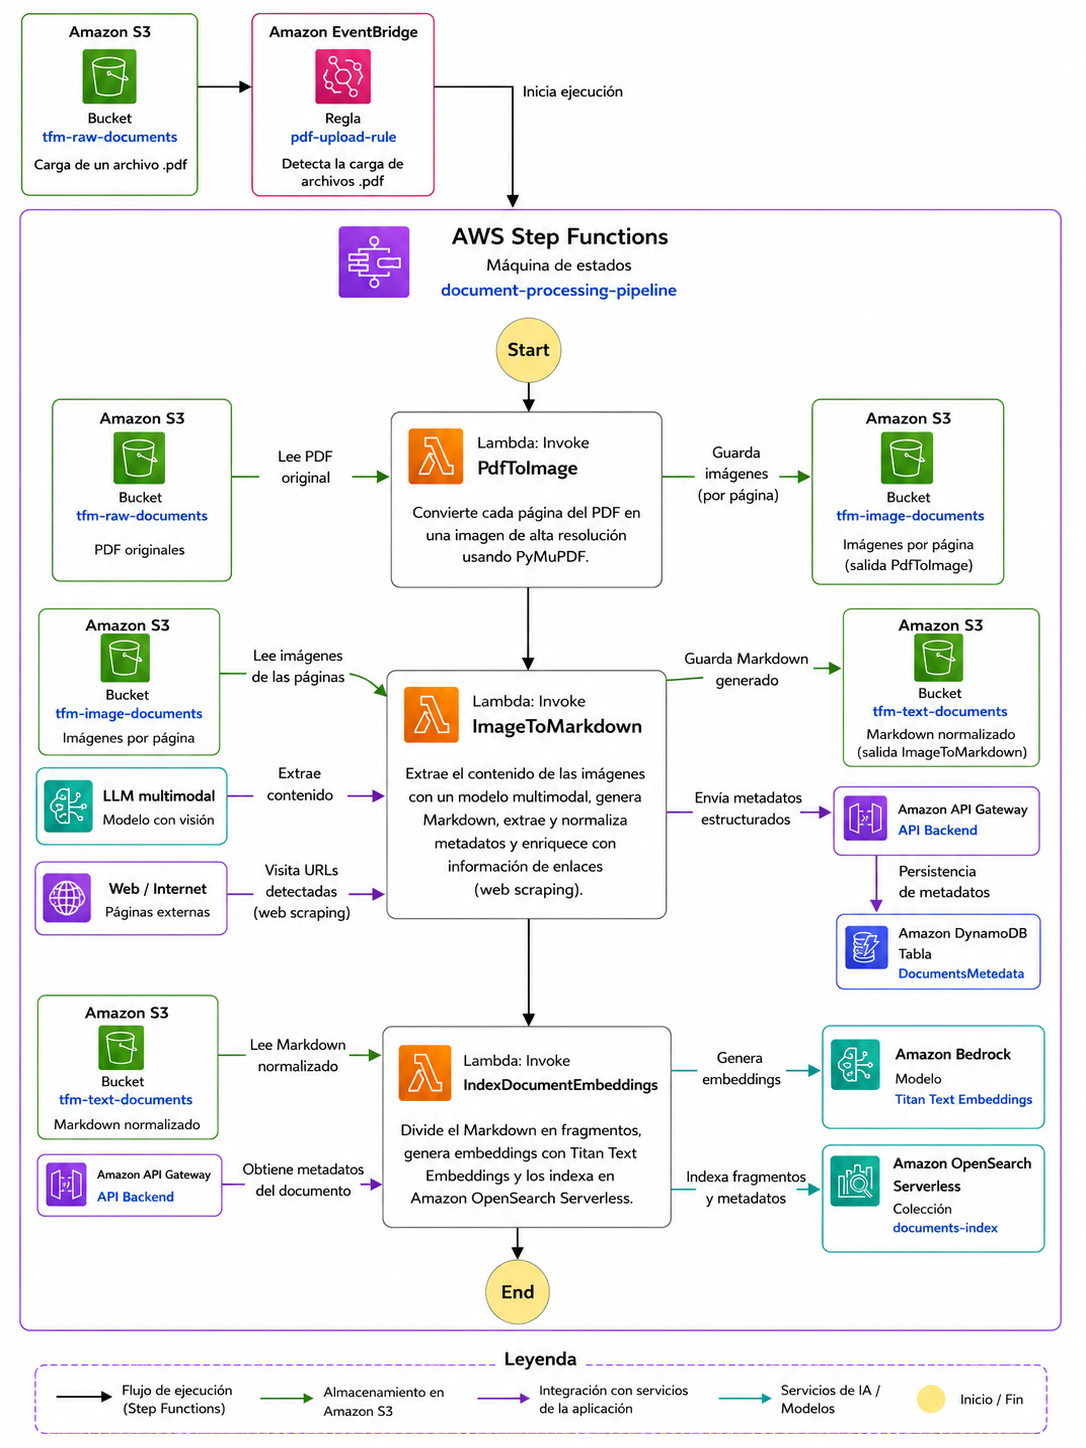
\includegraphics[width=1\textwidth]
    {assets/diagrama_pipeline_procesamiento_documental.png}
    \caption{Orquestación e interacciones del pipeline documental implementado mediante AWS Step Functions.}
    \label{fig:step-functions-document-pipeline}
\end{figure}

\begin{tfmbullets}

\item \textbf{\texttt{PdfToImage}.}
Recibe el PDF de Amazon S3 y renderiza cada página como una imagen de alta resolución
con PyMuPDF, conservando tablas, columnas, logotipos y precios que una extracción de
texto convencional podría perder. Las imágenes se almacenan de nuevo en S3 y sus claves
se incorporan al estado de la ejecución.

\item \textbf{\texttt{ImageToMarkdown}.}
Procesa cada imagen con un modelo multimodal que reconstruye el documento en formato
Markdown, conservando encabezados, tablas, condiciones y precios; si detecta enlaces
web, incorpora también esa información mediante \textit{web scraping}. A continuación
normaliza el contenido y extrae de forma estructurada los metadatos (destino,
proveedor, actividades, precios, condiciones, accesibilidad), incluyendo reglas para
unificar topónimos con distinta denominación y para no generar datos de contacto que no
aparezcan literalmente en el documento. El Markdown se almacena en S3 y los metadatos se
envían a la API backend, que los persiste en DynamoDB.

\item \textbf{\texttt{IndexDocumentEmbeddings}.}
Recupera el Markdown normalizado y sus metadatos, divide el contenido en fragmentos de
tamaño acotado y genera una representación vectorial de cada uno mediante Titan Text
Embeddings (Amazon Bedrock). Fragmentos, vectores y metadatos de destino y actividades
se indexan en Amazon OpenSearch Serverless.

\end{tfmbullets}

AWS Step Functions garantiza que cada función se inicie solo cuando la anterior ha
finalizado correctamente, y la persistencia de resultados intermedios en S3 permite
probar o reejecutar cada etapa de forma independiente. Al finalizar
\texttt{IndexDocumentEmbeddings}, el documento queda disponible para el sistema RAG sin
intervención manual desde la carga del PDF.

\TFMSection{Implementación del sistema RAG}

El sistema RAG fundamenta las respuestas en la documentación real de los proveedores,
reduciendo el riesgo de información inventada, desactualizada o ajena al destino
solicitado.

La base de conocimiento se implementa sobre Amazon OpenSearch Serverless: cada
fragmento se almacena con su representación vectorial, su contenido textual y los
metadatos extraídos en el pipeline (ciudad, provincia, país, actividades). Cuando un
agente consulta, la petición se transforma en un embedding (Titan Text Embeddings) y el
cliente RAG ejecuta en OpenSearch una búsqueda \textit{k-NN} combinada con filtros
exactos de destino y provincia, recuperando los fragmentos más próximos sin mezclar
documentación de otras localizaciones.

La Figura~\ref{fig:rag-query-flow} resume el flujo de consulta implementado, desde la generación del embedding hasta la construcción del contexto enviado al modelo de lenguaje.

\begin{figure}[htbp]
    \centering
    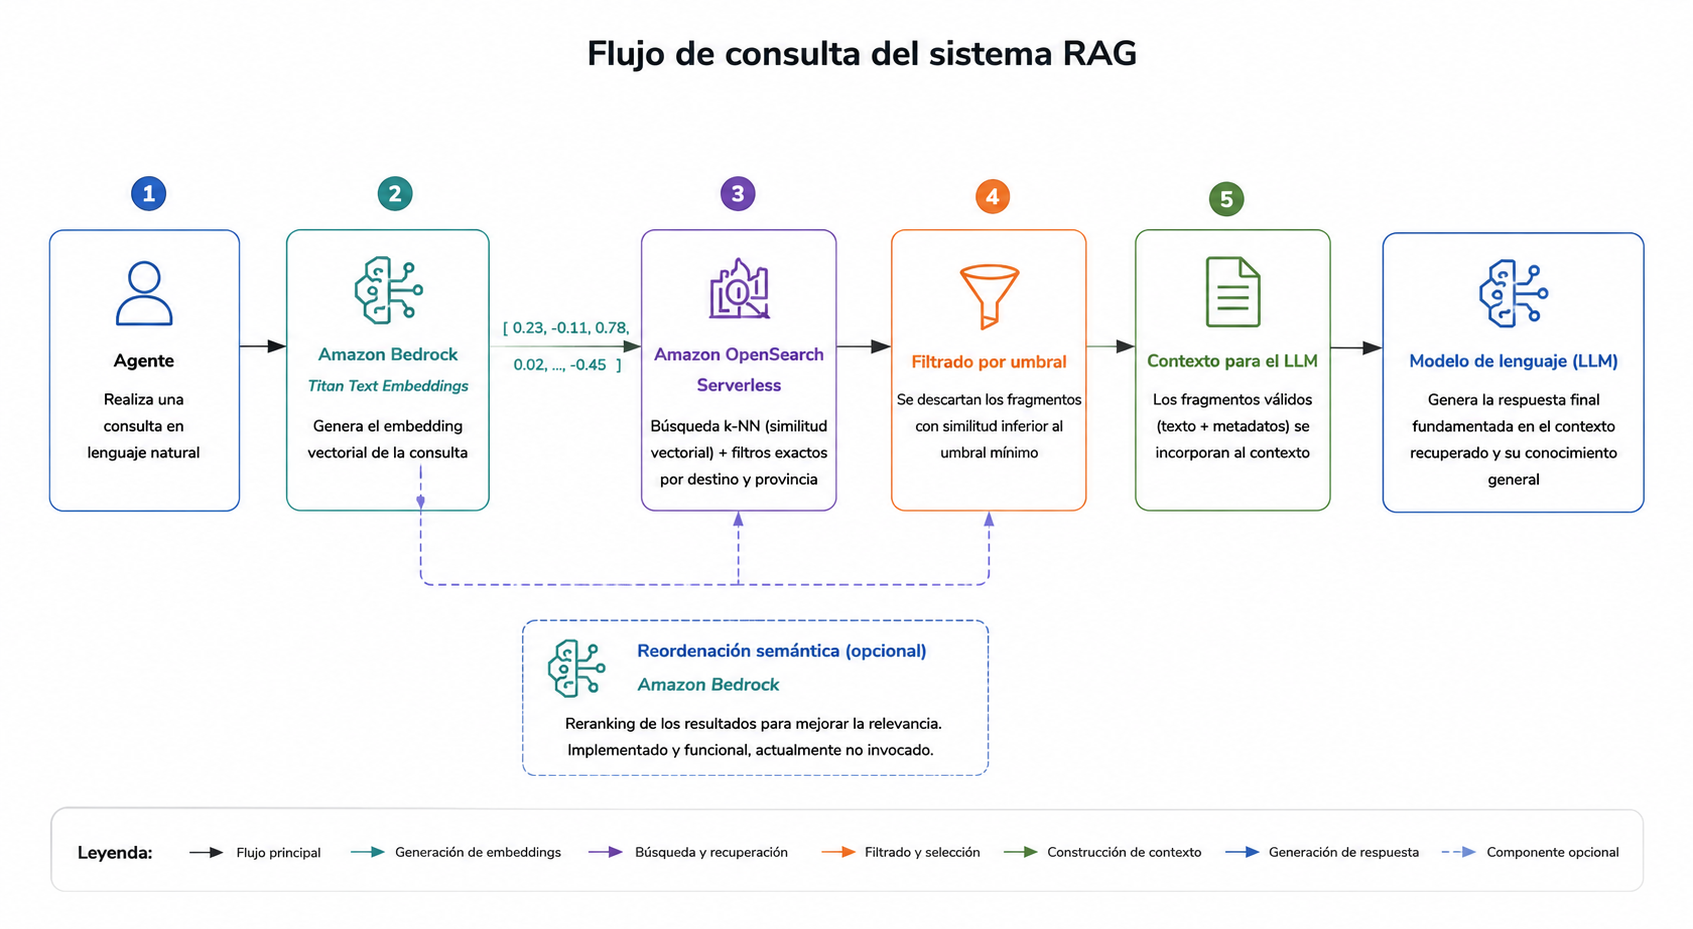
\includegraphics[width=0.75\textwidth]
    {assets/flujo_consulta_sistema_rag.png}
    \caption{Flujo simplificado de consulta del sistema RAG.}
    \label{fig:rag-query-flow}
\end{figure}

Las comunicaciones con Bedrock y OpenSearch Serverless usan credenciales y permisos de
AWS IAM, firmando las peticiones a OpenSearch mediante AWS Signature Version 4 para
evitar credenciales específicas de la base de datos dentro de la aplicación. Tras
recuperar los resultados, se aplica un umbral mínimo de relevancia que descarta los
fragmentos de baja similitud antes de incorporarlos al contexto del modelo.

El sistema dispone también de un módulo de \textit{reranking} sobre Amazon Bedrock, implementado y funcional pero aún no invocado en la ruta activa de consulta, a la espera de evaluar su impacto en calidad, latencia y coste. Los principales consumidores del RAG son el agente de información (contexto cultural y actividades) y, de forma complementaria, el agente de precios (alojamientos y servicios de la documentación de proveedores).

\TFMSection{Implementación del sistema multiagente}
\label{sec:impl-multiagente}

El sistema multiagente se implementa como un grafo de estados en LangGraph, cuyos nodos y flujos de control se resumen en la Figura \ref{fig:orquestrador}. A continuación se describe la función que cumple cada agente dentro del grafo y las decisiones de implementación adoptadas en cada caso.


\subsection{Agente orquestador}
Es el punto de entrada de cada conversación: analiza cada mensaje del profesional y extrae de forma estructurada los datos necesarios (cliente, origen, destino, fechas e intereses), solicitando una aclaración cuando falta información en lugar de generar una propuesta incompleta. Si el profesional cambia de destino a mitad de conversación, descarta automáticamente la información y los precios ya recopilados para evitar mezclar datos de dos viajes; si solo cambian las fechas, conserva el contexto cultural y solo recalcula precios. Antes de activar al resto de agentes, confirma en lenguaje natural los datos entendidos (por ejemplo, \textit{``He recibido toda la información necesaria para el viaje del Colegio Jesuitas a Alicante. Estoy comenzando el proceso de generación del folleto promocional.''}), para que el profesional pueda corregir la interpretación antes de que el sistema invierta tiempo generando la propuesta.

\begin{figure}[h!]
    \centering
    \makebox[\textwidth][c]{%
        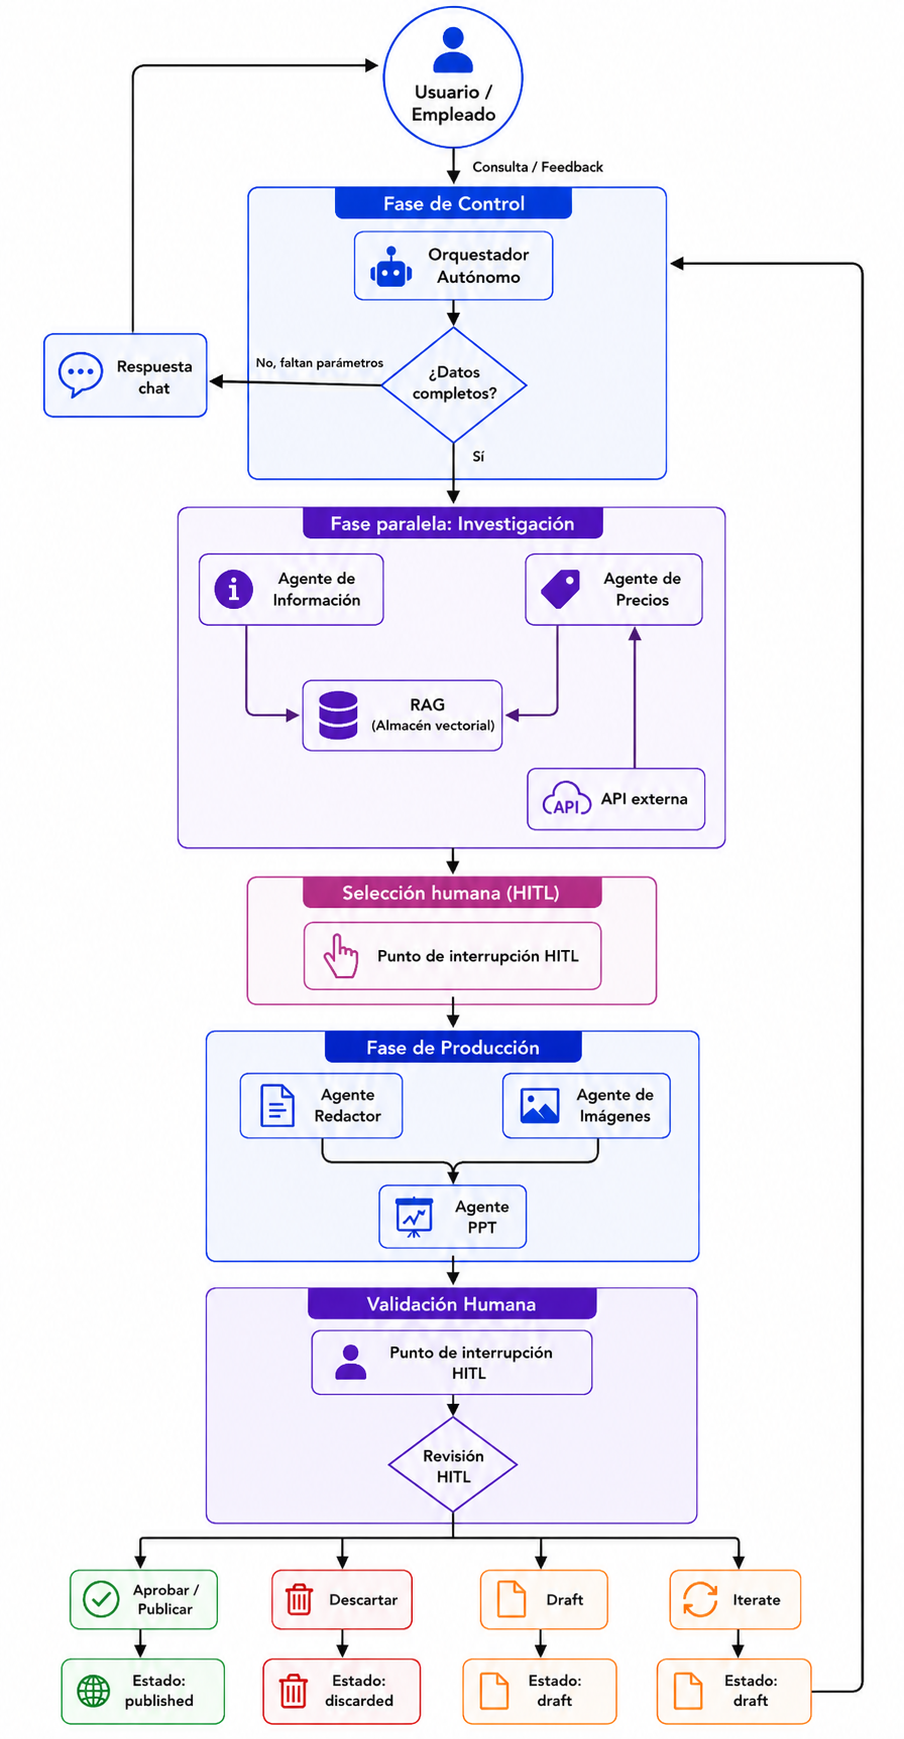
\includegraphics[
            width=1.3\textwidth,
            height=0.88\textheight,
            keepaspectratio
        ]{assets/diagrama_orquestrador.png}
    }
    \caption{Diagrama del orquestador multiagente.}
    \label{fig:orquestrador}
\end{figure}


\subsection{Agente de información}
Recupera, para el destino y cada interés expresado por el cliente, los fragmentos más relevantes de la base documental, descarta los que no superan un umbral mínimo de relevancia y sintetiza el resultado en un contexto cultural y un listado de actividades recomendadas, evitando la búsqueda manual y fundamentando la respuesta en contenido real en lugar de conocimiento genérico del modelo.

\subsection{Agente de precios}
Combina un servicio externo de precios de mercado en tiempo real con la base documental (para alojamientos que solo aparecen en catálogos de proveedores). La selección de candidatos (vuelos más económicos, alojamientos mejor valorados) se calcula de forma determinista en código, no con el modelo de lenguaje, garantizando un orden siempre coherente y verificable. El resultado no se aplica automáticamente: se presentan varias opciones de cada categoría para que el profesional elija (Figura~\ref{fig:manual-seleccion-precios}), manteniendo la decisión comercial en manos humanas.

\subsection{Generación del itinerario}
A partir de la información recuperada, los precios seleccionados y las preferencias de la conversación, se genera un itinerario día a día. Varios cálculos que podrían delegarse en el modelo se resuelven en código para garantizar su exactitud: duración del viaje a partir de las fechas, y horarios de vuelo incorporados como instrucción al itinerario en lugar de dejar que el modelo los interprete en formato libre. El itinerario respeta además un límite de extensión calculado según el espacio disponible en la plantilla, para que el texto encaje sin retoque manual.

Cada jornada se redacta en tres bloques (Mañana, Tarde y Noche), combinando logística práctica con recomendaciones ancladas en la documentación recuperada. En una propuesta real para un grupo escolar, el sistema incorporó una condición de precio para grupos extraída de la documentación de un proveedor (\textit{``para grupos +20 la entrada es 4€ p/p''}), mostrando que la personalización traslada al itinerario condiciones comerciales del tipo de cliente cuando están disponibles.

\subsection{Generación de la propuesta comercial}
La propuesta combina dos elementos generados de forma independiente --una imagen de portada \parencite{openai-images-2025} y el itinerario-- integrados en una plantilla corporativa PPTX editable, ajustando dinámicamente el número de diapositivas según la duración del viaje. El resultado es un documento ya maquetado y listo para revisar o enviar, sin intervención de diseño. La propuesta incorpora además, junto al precio, un apartado de condiciones comerciales (qué queda excluido y la sujeción a disponibilidad, viajeros y fecha de reserva; Figura~\ref{fig:manual-revision-flyer}), evitando que el profesional deba añadirlas manualmente.

\subsection{Gestión del estado y transiciones}
Todos los agentes comparten un mismo estado (parámetros del viaje, información recuperada, precios, itinerario y resultado de cada etapa), que se conserva de forma persistente en cada decisión humana, permitiendo interrumpir una propuesta y retomarla más adelante sin perder el trabajo realizado. Las cuatro acciones de la revisión final (Figura~\ref{fig:manual-revision-flyer}) --aprobar, rechazar, descartar o guardar como borrador-- se corresponden directamente con los valores del estado de revisión.

Con fines de depuración, la barra lateral incorpora un panel \textit{State Inspector} (Figura~\ref{fig:manual-seleccion-precios}) que expone en JSON el historial de mensajes del grafo; no forma parte del flujo del profesional, pero ha sido útil para verificar que el estado persiste correctamente entre interrupciones.

Como observación técnica honesta, el \textit{checkpointing} en memoria (\texttt{MemorySaver}) no conserva la posición exacta del \texttt{interrupt} tras un reinicio del proceso, por lo que una heurística infiere el punto de interrupción a partir del propio contenido persistido (por ejemplo, precios candidatos sin selección o un borrador ya redactado). Esta heurística resuelve el caso práctico, pero la persistencia externa del estado conversacional interrumpido se mantiene como trabajo futuro prioritario (Capítulo 8).

\TFMSection{Observabilidad y trazabilidad (LangSmith)}
Para dar cumplimiento al requisito RNF7 (Trazabilidad), se ha incorporado \textbf{LangSmith} como plataforma de observabilidad, integrada mediante un módulo propio (\texttt{src/observability.py}) que actúa como capa fina sobre el trazado automático de LangChain y LangGraph.

La integración es opcional y no invasiva: solo se activa con \texttt{LANGSMITH\_TRACING=true} y una \texttt{LANGSMITH\_API\_KEY} válida, de forma que un entorno sin la clave configurada sigue funcionando en silencio; desactivada, el módulo es un no-op transparente para el resto del código.

Cuando el trazado está activo, cada ejecución del grafo se enriquece con información de negocio que, de otro modo, quedaría invisible en un panel de trazas genérico:

\begin{tfmbullets}
\item \textbf{Metadatos por propuesta:} cada ejecución se etiqueta con el identificador de la propuesta (\texttt{flyer\_id}) y el nombre del cliente, de forma que el panel de LangSmith permite localizar y filtrar las trazas de una conversación concreta en lugar de mostrar un flujo anónimo.
\item \textbf{Metadatos por agente:} cada llamada al modelo de lenguaje dentro de un agente se etiqueta adicionalmente con el nombre del propio agente (\texttt{agent:orchestrator}, \texttt{agent:pricing\_agent}, etc.), heredando las etiquetas y metadatos de la ejecución padre, lo que permite desglosar coste, tokens y latencia por agente dentro de una misma propuesta.
\item \textbf{Nombres de ejecución legibles:} cada traza recibe un nombre descriptivo (por ejemplo, \textit{``Flyer generation — Cliente X''}) en lugar del identificador interno del grafo, facilitando la inspección manual del panel durante el desarrollo y la evaluación del sistema.
\end{tfmbullets}

Esta capa se ha propagado a los agentes orquestador, información, precios e imagen y al propio grafo (\texttt{src/graph.py}), con pruebas unitarias dedicadas (\texttt{tests/unit/src/test\_observability.py}) que verifican tanto el no-op como el enriquecimiento correcto de metadatos \parencite{langsmith2026docs}.

\TFMSection{Integración con modelos de lenguaje}
Cada agente utiliza el modelo de lenguaje más adecuado a su tarea, atendiendo a un equilibrio entre coste y fiabilidad: modelos con cuota de uso económica para tareas de alto volumen (interpretación de la conversación, reconocimiento de documentos) y modelos con mayor capacidad de generación estructurada para tareas donde un error tiene más impacto en el resultado final (recuperación de información, cálculo de precios, redacción del itinerario). En todos los casos se exige al modelo una salida estructurada validada contra un esquema de datos predefinido, en lugar de interpretar texto libre, lo que evita errores de formato en las respuestas y hace que el comportamiento del sistema sea predecible y verificable.

\TFMSection{Integración con fuentes externas}

La base documental no siempre incluye precios actualizados de vuelos y alojamientos, por lo que el agente de precios se integra con SearchAPI, un servicio externo que consulta Google Flights y Google Hotels mediante API REST \parencite{searchapi2026flights,searchapi2026hotels}.

Para vuelos se lanzan en paralelo dos consultas independientes (ida y vuelta), lo que reduce el tiempo de respuesta y permite combinar aerolíneas distintas cuando resulta más económico; los resultados incluyen aeropuertos, horarios, duración, escalas y precio. Para alojamientos se consulta por destino, fechas y número de viajeros, normalizando nombre, valoración, precio y datos de la estancia. Ambos resultados se transforman en modelos internos comunes, de forma que el resto de la aplicación no depende de la estructura de SearchAPI y sería posible sustituir o añadir proveedores sin tocar la interfaz ni el flujo multiagente.

Durante el desarrollo se estudió primero integrar Amadeus mediante un servidor MCP, descartado por los cambios en su plataforma Self-Service y la imposibilidad de mantener un acceso gratuito adecuado para la prueba de concepto \parencite{amadeus2026developers}; SearchAPI permitió completar la integración con menor complejidad de acceso.

Al tratarse de datos orientativos que pueden variar hasta la reserva efectiva (Capítulo~2), el sistema presenta varias alternativas al profesional y mantiene la selección final
como un punto obligatorio de intervención humana.

\TFMSection{Implementación de la API}
La API de persistencia expone los servicios que permiten a la interfaz y al pipeline documental compartir una única fuente de verdad: autenticación de usuarios, metadatos documentales y estado de las propuestas. Los usuarios finales se autentican con un token de sesión y el pipeline con una cuenta de servicio independiente, de forma que las credenciales de un empleado nunca se comparten con procesos automáticos. Una propuesta solo puede modificarla quien la creó, aunque su consulta desde el histórico está abierta a cualquier usuario autenticado, acorde al uso compartido de un equipo comercial.

\TFMSection{Implementación del frontend}

La interfaz se ha desarrollado en Streamlit como una aplicación conversacional orientada al personal interno de una agencia de viajes, ocultando la complejidad del sistema multiagente y presentando solo la información y decisiones necesarias en cada fase.

Se organiza en dos vistas: la de conversación, desde la que el usuario describe el viaje en lenguaje natural y el orquestador extrae los parámetros y activa el resto del flujo; y el histórico, con los viajes generados por el equipo, su estado y su información asociada en formato tabular. Tras iniciar sesión, el usuario puede iniciar una conversación, consultar o retomar propuestas anteriores, o descargar una propuesta en PPTX.

La interfaz implementa también los dos puntos de interacción humana del diseño: tras la consulta de precios, para seleccionar manualmente vuelo y alojamiento (o indicar que el cliente viaja por sus propios medios); y tras generar la propuesta comercial, para aprobarla, solicitar modificaciones, descartarla o guardarla como borrador, actualizando el estado compartido del grafo.

Todas las capturas de pantalla y el flujo de uso paso a paso se recogen en el
Anexo~\ref{anexo:manual-aplicacion}.

\TFMSection{Despliegue e Infraestructura en AWS}

La solución se ha desplegado sobre una arquitectura híbrida en AWS, combinando
servicios \textit{serverless} para el procesamiento documental y la persistencia con una
instancia de ejecución permanente para la aplicación conversacional, tal como resume la
Figura~\ref{fig:aws-infrastructure}.

\begin{figure}[htbp]
    \centering
    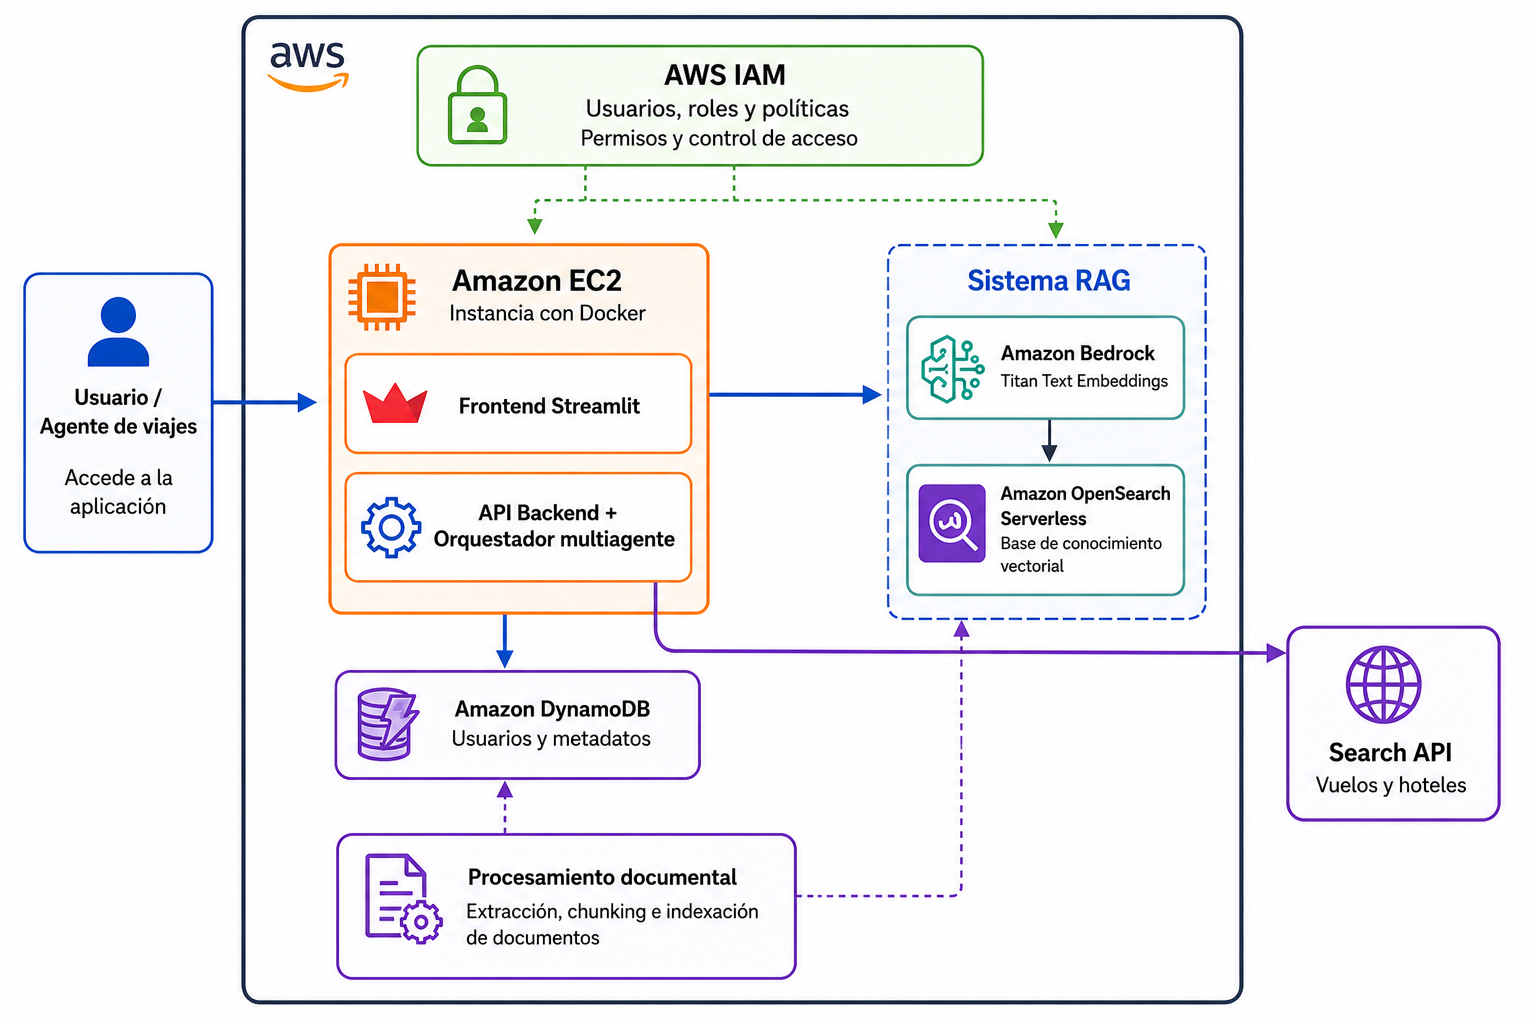
\includegraphics[width=1\textwidth]
    {assets/diagrama_infra_aws.png}
    \caption{Arquitectura general de despliegue de la solución en AWS.}
    \label{fig:aws-infrastructure}
\end{figure}

Amazon S3 actúa como repositorio documental principal, con buckets separados para
documentos originales, imágenes por página y Markdown normalizado, conservando
resultados intermedios y desacoplando las etapas. Amazon DynamoDB implementa la
persistencia estructurada (usuarios, metadatos documentales y estado de las
propuestas), centralizada a través de la API backend en FastAPI. La base de
conocimiento RAG se implementa sobre Amazon OpenSearch Serverless, con Amazon Bedrock
generando los embeddings (Titan Text Embeddings) y el módulo opcional de reranking.

La interfaz en Streamlit, el orquestador multiagente y la API backend se ejecutan en
una instancia Amazon EC2 mediante Docker y Docker Compose, lo que permite servicios de
larga duración, conservar el estado de las conversaciones mientras la aplicación está
activa, y actualizar cada componente reconstruyendo su contenedor. El sistema consulta
además SearchAPI, de forma separada de los servicios internos de AWS.

El acceso a los recursos se controla mediante AWS IAM, con usuarios, roles y políticas
diferenciadas por tarea (administración, despliegue, ejecución) y permisos mínimos para
cada función Lambda y servicio interno, manteniendo las credenciales de los usuarios de
la aplicación separadas de las identidades de los procesos automáticos.

La infraestructura se ha configurado manualmente en la consola de AWS, lo que ha
permitido validar la arquitectura completa dentro del alcance de la prueba de concepto
pero reduce su reproducibilidad y dificulta auditar los cambios; la definición mediante
\textit{Infrastructure as Code} se plantea como línea prioritaria de trabajo futuro.

\TFMSection{Seguridad y gestión de errores}
El sistema incorpora varios mecanismos para tolerar fallos sin interrumpir la experiencia del profesional: reintentos automáticos ante errores transitorios de los proveedores de modelos de lenguaje, y una degradación controlada cuando el sistema RAG o las fuentes externas de precios no están disponibles, de forma que el flujo continúa (por ejemplo, sin contexto documental o sin precios de una fuente) en lugar de interrumpirse por completo. Esta decisión es especialmente relevante en un sistema orientado a un caso de uso comercial, donde una propuesta incompleta pero disponible resulta más útil que un error que bloquee todo el proceso.
